\chapter{Bayesian Networks, Causality and the
Passage of Time}
%\addcontentsline{toc}{chapter}{Bayesian Networks, Causality and the Passage of Time}

\label{ch-bnets-time}

This chapter is based
on a blog post (see Ref.\cite{bnets-passage-time})
from my blog \qt{Quantum Bayesian Networks}.

\section{Unifying Principle of this book}
The unifying principle of this
book is Bayesian Networks (bnets).
The main goal of this book
is to explain
as much of Artificial Intelligence (AI)
and Machine Learning (ML)
as possible
using bnets.

Bayesian Networks are a graphical representation of the chain rule for
conditional probabilities.
 They are not a \qt{heuristic algorithm} like XGBoost or Neural Nets.
They are a very simple, intuitive, basic and general definition. I would say
that the definition of a Bayesian Network is as important to Probability
Theory as the definition of a Group is to Abstract Algebra. Algebraic groups
are never going to go out of fashion and neither are B nets.

An Artificial Neural Net can be defined as a Bayesian Network with a layered
structure, and such that all its nodes are deterministic\footnote{Neural Nets (NNs)
are DAGs, but they contain a lot of 
spurious arrows whose direction
or very existence has no causal motivation,
and they could be missing
other arrows which 
would have a causal motivation.
 So I like to
say that NNs are acausal DAGs.}. A decision tree
 can be trivially converted into a
B net that has the same tree structure (for more details about
this conversion, see the Chapter \ref{ch-dtree} on decision trees).
The SCM diagrams favored by Pearl are just bnets
whose internal nodes are deterministic and external ones
are probabilistic.
In fact, as I show in this book, most methods in AI can be
understood in terms of B nets---just
like many theorems in Abstract Algebra
can be understood in terms of groups.



\section{You say tomato, I say tomato}
In this chapter, I will use the terms Bayesian Network
(bnet), causal model and DAG as if they were synonymous.
My justification for doing this is as follows.


 A Bayesian Network is a DAG + probability tables. One can easily compute the
 probability tables from DAG + Dataset. Therefore,

You say DAG+Dataset, I say Bayesian Network.

The use of the terms \qt{causal model} and \qt{DAG}, as an
alternative to the term
\qt{Bayesian Network}, has become popular in the last decade
among economists, epidemiologists,
AI researchers and even Judea Pearl himself. It seems some
people think \qt{causal models} and \qt{DAGs} are revolutionary,
whereas Bayesian
Networks are a concept that was tried 25 years ago, and has been replaced
since then by stuff that works better. But any time you have a Dataset, which
is almost always true in practice in Economics,
Epidemiology  and AI, a DAG implies a
Bayesian Network and vice versa.



\section{A dataset is causal model free}
Time and time again, Judea Pearl makes the point on Twitter to neural net
advocates that they are trying to do a provably impossible task,
 to derive a
causal model from data. I could be wrong, but this is what I think he means.

When Pearl says \qt{data}, he is referring to what is commonly called a
dataset.
A {\bf dataset} is a table of data, where all the entries of each column have
the
same units, and measure a single feature, and each row refers to one
particular sample or individual. Datasets are particularly useful for
estimating probability distributions and for training neural nets. When Pearl
says a \qt{causal model}, he is referring to a DAG (directed acyclic
graph) or a
bnet
(Bayesian Network= DAG + probability table for each node of DAG).

Sure, you can try to derive a causal model from a dataset,
 but you’ll soon find
 out
that you can only go so far.

The process of finding a partial causal model from a dataset is called
structure
learning (SL).  SL can be done quite nicely with Marco Scutari’s open source
program bnlearn. There are 2 main types of SL algorithms: score-based and
constraint based. The first and still very competitive constraint-based SL
algorithm was the Inductive Causation (IC) algorithm proposed by Pearl and
Verma in 1991. So Pearl is quite aware of SL. The problem is that SL often
cannot narrow down the causal model to a single one.
It finds an undirected
graph
(UG), and it can determine the direction of some of the arrows in the UG, but
it is often incapable, for well understood fundamental
---not just technical---
reasons, of finding the direction of ALL the arrows of the UG. So it often
fails to fully specify a DAG model.

Let’s call the ordered pair
(dataset, causal model) a
dataset++ . Then what I
believe Pearl is saying is that a
dataset is causal model-free or causal model-less
(although sometimes one can find a partial
causal model hidden in there). A dataset
is not a dataset++.

{\bf Caveat to this section:} Define a {\bf time-series table (TST)} to be
a table of data, where all the entries of each column have
the
same units, and measure a single feature at different times with time increasing down the table.
Hence, the rows of a TST are chronologically ordered (they 
specify a time series)
whereas those of a dataset aren't. Whereas it is not possible to
fully specify a DAG from a dataset alone, it is possible
to do so from a TST. See the python app CausalFit (Ref.\cite{CausalFitbit}) for a possible
way extracting a causal DAG from a Fitbit TST.

\section{What is causality?}
What is Causality, really, and how do Bayesian Networks
(a.k.a. Causal Models,
DAGs) encode it?
For me, Causality is a time-induced ordering between two events, the
transmission of information (and its accompanying
energy) from the earlier of the two events to the later
one, and the physical response of the later event to the reception of that
information. 

Note that this definition
of causality does not mention
correlation.
It is often assumed that even though
correlation does not imply causation,
causation implies correlation.
But the latter statement is false; there
are scenarios, albeit  unusual,
\qt{fine tuned} ones,
in which there is causation
without correlation.
For example, 
consider a bnet 
with arrows $\rvx\rarrow \rvy$
and $\rvx\rarrow \rvc \rarrow \rvy$.
When we amputate 
the arrows entering $\rvx$,
a dependence
between $\rvx$ and $\rvy$ persists,
so we say $\rvx$ causes $\rvy$.
Even
though $\rvx$ causes $\rvy$,
it's possible to tune the 
probabilities
of the bnet so that
the effect of the path $\rvx-\rvc-\rvy$
and the effect of the direct path $\rvx-\rvy$
cancel 
each other out and
produce zero 
correlation between $\rvx$ and $\rvy$.
As a trivial example, suppose
$\rvc=2\rvx$, $\rvy=\rvc-2\rvx=0$.
Since $\rvy=0$, it's uncorrelated with $\rvx$.

The nodes of a bnet represent random variables. Some of those
random variables are clearly events (i.e., they occur at a definite time).
For example, let D=0 if a patient is not given a drug, D=1 if he/she is given
it. D occurs at a definite time. But other random variables represent
qualities which do not occur at a definite time. For example,
G=gender=male, female. G does not occur at a definite time.  But even in the
case of a quality like G, its value is first decided at birth, so one can
ascribe to G a particular, albeit fuzzy time interval during which it is
decided. If M=0(single), 1(married), then we can assign to M the day of the
marriage. Both the time interval assigned to G and to  M are somewhat
ambiguous, but still, most people would say that G occurs before M (if a
marriage occurs at all). Saying the opposite, that M occurs before G, seems
pretty hard to understand. If two nodes A and B of a bnet have time intervals
ascribed to them such that the time interval of A does not clearly occur
before or after the time interval of B, and if also there is a large causal
correlation between A and B, then it probably does not matter
much whether one draws an arrow from A to B, or the opposite.

Now that we understand that the arrows in a bnet really do encode the
direction of time, it becomes clear why a dataset does not fully specify a
bnet. By a dataset (think of a dataframe in Pandas or R), I mean an array of
numbers where the columns refer to features and the rows refer to individuals
in a population. The column labels of the dataset become the node names of
the bnet. Nowhere in a dataset is there any indication of the time ordering
of the features. Hence, it’s impossible to create, from a dataset alone, a
bnet, because bnets do carry such time-ordering information.

Chapter \ref{ch-granger-c} discusses
 Granger Causality
(GC). The critics of GC point out that it assumes, somewhat erroneously,
that if event A precedes B and the two events are correlated, A must
cause B. I agree. Most roosters crow in response to the stimulus of the
sunrise light.  A rooster could crow before sunrise if,  for example,  he
had an alarm clock that woke him up 30 minutes before sunrise, but such cases
are uncommon, and seem to involve other intermediate events.  The moral is
that time ordering and correlation are not sufficient
conditions for causality. To establish causality with more certainty, one
also needs a pinch of prior expert knowledge, or one must gain that expert
knowledge through \qt{do} operator experimentation.



\section{Bayesian Networks and the passage of time}

Now that we understand that a bnet’s arrows are encoding roughly the passage
of time, it becomes possible to glean from this insight a simple method,
which, although not very rigorous, is really helpful to me. I will illustrate
said method with the famous \qt{Asia} bnet in Fig.\ref{fig-asia}.
 In this bnet, all nodes
have two  possible values, 0 and 1.

\begin{figure}[h!]
\centering
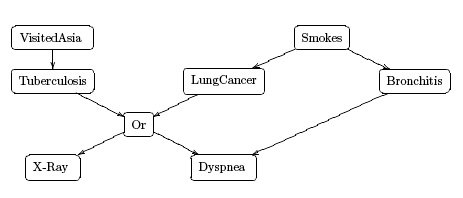
\includegraphics[width=5in]
{bnets-time/asia.jpg}
\caption{Asia bnet. Dyspnea=trouble breathing}
\label{fig-asia}
\end{figure}


Given a dataset for this bnet, one can calculate the correlation between
every 2 features of the dataset. The feature names become the node names, and
links are drawn between any 2 nodes whose correlation is 
causal and greater in absolute
value to some threshold value.
This gives an undirected graph that can be
obtained from bnet Fig.\ref{fig-asia}
 by erasing the directions of the arrows. So how
can we guess the directions of the arrows? Well, one uses a little bit of
\qt{expert knowledge} to conclude that

time(Visited Asia) $<$ time(Tuberculosis) $<$ time(Or) $<$ time(X-Ray,
Dyspnea)

Also

time(smokes) $<$ time(LungCancer, Bronchitis) $<$ time(Or) $<$ time(Dyspnea)

If time(A) $<$ time(B), then A $\rarrow$ B. Like I
said before, the times we ascribe to
these events are somewhat fuzzy and open to debate, so this algorithm is far
from being rigorous. But often, saying that  time(A)$<$time(B) makes much more
sense than saying that time(B)$<$time(A). When in doubt about the best
direction to give to an arrow of an undirected graph, I recommend calculating
a Goodness of Causal Fit metric (see Chapter
\ref{ch-good-causal-fit}) which makes use of \qt{do} operator
experimentation.


A dataset cannot fully specify a
bnet because it lacks time ordering info. A dataset also cannot do the harder
task of specifying a bnet that is a good causal fit to the problem, because
it lacks time ordering info AND prior expert knowledge AND expert knowledge
gained from posterior \qt{do} operator experimentation.

\section{Advice for the DAG-phobic}
\label{sec-advice-dagophobic}

DAGs are your friends. DAGs should be easy and fun to dream up. After all, I
am convinced that DAGs are an integral part of how humans think, so they
should come naturally to us.  Nevertheless, many people are scared of, or
detest, DAGs. I think it’s because they fail to grasp the following 3 things:

1. DAGs are not unique. Stop thinking that you have to find the unique DAG
for the situation being considered. You just have to find a DAG that is a
good causal fit for the situation. If a DAG is too complicated, you can
always simplify it by merging several nodes into a single more abstract one,
or by summing over unwanted nodes.

2. The nodes of a DAG are roughly ordered from past to present. The arrows of a DAG roughly
reflect the passage of time.

3. DAGs represent scientific hypotheses that can and should be tested with
do experiments. Causal Inference is an
application of the scientific method, which consists
of the following steps:
formulate hypothesis (DAG), devise experiment
to test it, test it.
